\documentclass[10pt,dvipdfmx]{standalone}
% \documentclass[dvipdfmx,b5paper,papersize]{jsarticle}
\usepackage{tikz}
\usetikzlibrary{intersections, calc}

\begin{document}

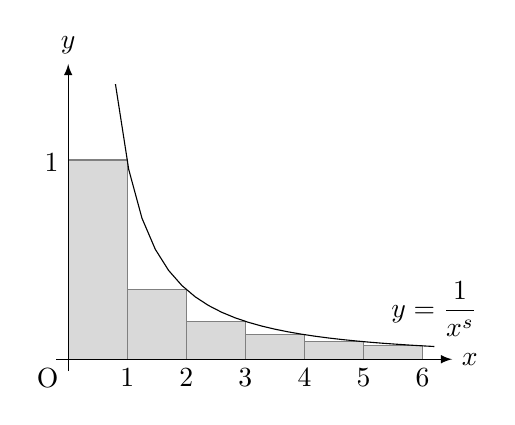
\begin{tikzpicture}[x=0.75cm,y=2.5cm,>=latex]
  \def\width{1.0};
  \def\s{1.5};
  \def\n{6};
  \def\domain{0.8:\n*\width+0.2};
  \def\fx{{((\x*\width)^-\s)}};

  \node(O) at (0,0) [below left]{O}; % 原点
  \path [name path=graph, domain=\domain] plot(\x, \fx);
  \foreach \x in {0,...,\n} {
    \path[name path global/.expanded=path-\x](\width+\width*\x,0) -- (\width+\width*\x,1.1); % 縦棒。関数によって範囲を調整。足りないとエラー、長すぎると図の上に空白が。
    \path[name intersections={of=graph and path-\x}]; % 交点求める
    \coordinate (p-\x) at (intersection-1); % 交点
    \filldraw[fill=gray!30,draw=gray] ($(0,0)!(p-\x)!(1,0)$) rectangle ($(p-\x)+(-\width,0)$); %長方形を描く
  }
  \foreach \x in {1,...,\n} { % x軸目盛り
    \node(O) at (\x*\width,0) [below]{$\x$};
  }
  \node(O) at (0,1) [left]{$1$}; % y軸目盛り
  \draw[->] (-0.2,0) -- (\n*\width+0.5, 0) node[right]{$x$};
  \draw[->] (0,-0.2*0.75/2.5) -- (0, 1.5) node[above]{$y$};
  \draw [domain=\domain] plot(\x, \fx) node[above]{$\displaystyle y=\frac1{x^s}$}; % 短冊の上に draw したいので、短冊drawコマンドの後に書く
\end{tikzpicture}

\end{document}